%!TEX root = ../../thesis.tex

The \ac{SM} of particle physics is a gauge quantum field theory describing the kinematics and interactions of sub-atomic particles \cite{Aitchison,Peskin}. The dynamics of such a 
theory are determined by the symmetries respected by the Lagrangian density.
The \ac{SM} is invariant under local transformations of the \SMgroup gauge group,
resulting in the strong, weak and electromagnetic forces of nature and determining
the particle content of the theory. Additionally, invariance under global 
transformations of the Poincaré group ensures the theory is identical in all 
inertial frames of reference, as asserted by special relativity.

Each gauge theory of the \ac{SM} describes the dynamics of a force of nature, which 
is mediated by a number of gauge bosons and couples to a conserved current, in 
accordance with Noether's theorem. \ac{QCD} describes the strong 
interaction, is mediated by eight gluons and couples to colour charge. \ac{QED}
describes the electromagnetic interaction, is mediated by the 
photon and couples to electric charge. The weak interaction is mediated by the massive 
\PWpm and \PZ bosons and is understood within the context of \ac{EW} theory,
a unification of the electromagnetic and weak interactions. A quantum field theory of
gravity is not included in the \ac{SM}. It is important to note that the gauge groups of 
the strong and weak interactions are non-abelian. Physically, this means that the
gauge bosons are themselves charged and therefore experience self-interactions.

\begin{figure}
	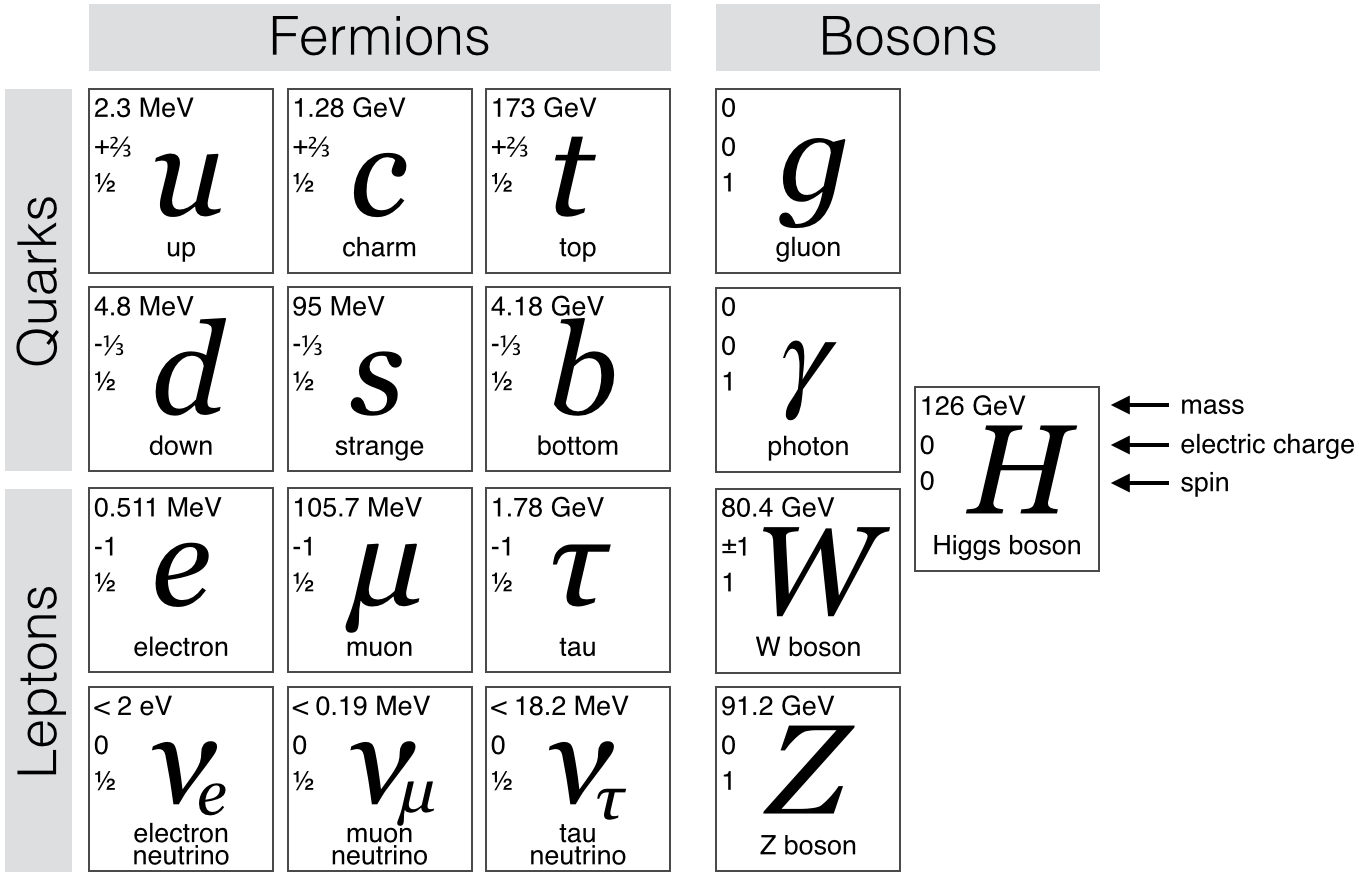
\includegraphics[width=\largefigwidth]{tex/motivation/sm_particles}
	\caption{The particle content of the \ac{SM}. Particle masses from \cite{PDG}.
	\todo[inline]{Should I remove the Higgs mass here?}}
	\label{fig:sm_particles}
\end{figure}

The elementary particles of the \ac{SM} are summarised in \Figure~\ref{fig:sm_particles}.
They are naturally separated into bosons (integer spin) and fermions (half-integer spin).
In addition to the gauge bosons previously introduced, the Higgs boson is a by-product
of electroweak symmetry breaking (described in \Section~\ref{sec:ewsb}) and its
couplings are proportional to mass. The twelve flavours of fermions are categorised 
according to the interactions they experience, or equivalently the charges they posses: 
quarks (strong, electromagnetic, weak), charged leptons (electromagnetic, weak) and 
neutrinos (weak). The fermions are also arranged in three generations of increasing
mass - the first generation are stable since they cannot decay to lower mass particles.
Most particles have an associated antiparticle with identical mass but inverted internal 
quantum numbers.
